\chapter{Evolutionary Algorithms} % top level followed by section, subsection

%: ----------------------- paths to graphics ------------------------

% change according to folder and file names
\ifpdf
    \graphicspath{{2/figures/PNG/}{2/figures/PDF/}{2/figures/}}
\else
    \graphicspath{{2/figures/EPS/}{2/figures/}}
\fi

%: ----------------------- contents from here ------------------------

%\begin{flushright}
%Life results from the non-random survival 
%\linebreak
%of randomly varying replicators.
%\linebreak
%Richard Dawkins 
%\end{flushright}
\section{Introduction - Overview}
A number of stochastic optimization methods based on the ideas presented in Darwin's theory of evolution on the origin of species \cite{Darwin} have been proposed. Hereafter, all these methods along with their variants will be referred to as Evolutionary Algorithms (EAs). The increased power of modern computational platforms and its availability with relatively low cost, combined with algorithms capable to exploit their capabilities,  allowed EAs to be routinely used as industrial design tools.     

An EA is a stochastic optimization method that maintains a population of individuals $P^g=(\vec{x}_1,...,\vec{x}_{\lambda}),~\lambda \ge 1$ for each generation $g$. Each individual $\vec{x}$ represents a potential solution to the optimization problem in hand and must be evaluated to obtain a measure of "fitness" or "cost", according to user-defined objective functions. Then, the population of the next ($g+1$) generation is formed by selecting the more fit individuals (to be referred to as parents) and evolve them by applying a number of evolution operators (recombination, mutation, etc.) that mimic the evolution of species. The new population (to be referred to as offspring) is expected to better fit to the environment as described by the objective functions.     

The first attempts to use EAs as problem solving techniques is dated back to mid-50s and can be found is separate works presented by Friedberg, Brernermann and Box. Friedberg cite(1958 and 1959) presented an EA aiming at creating a program to perform a given task; though quite premature, this was in fact an ancestor of evolutionary programming (see below). During the same period of time, Bremermann (cite Bremermann 1962) was among the first to apply EAs in numerical optimization problems, for linear and convex problems as well as the solution of nonlinear systems of equations. Box proposed the use of EAs as a method for improving industrial processes and, thus, increasing industrial productivity (cite Box 1957, Box and Draper 1969). By that time, these first attempts were treated with considerable skepticism. However, during the next decade, methods currently identified as the three main variants of EAs, namely evolutionary programming (EP), evolutionary strategies (ES) and genetic algorithms (GA), were clearly established.

EP was proposed by L. J. Fogel by mid-60s  (cite fogel 64,66,68). EP was developed by considering machine learning tasks by means of finite state machines (FSM\footnote{A finite-state machine (FSM) is a mathematical model used to design computer programs and digital logic circuits. FSM is an abstract machine that can be in one of a finite number of states.}). The optimization problem was  initially defined as evolving an algorithm (program) for predicting arbitrary time series.  In EP  \cite{Fogel}, offspring are created by randomly mutating each parent, each parent producing one offspring (initially). The offspring with the greatest payoff is, then, retained for becoming a parent in the next generation. EP was successfully applied to problems in prediction identification, automatic control and pattern recognition. Until mid-80s, EP was confined to the FSM representation. In 1986, though, EP was extended (Fogel and Fogel 1986) to alternative representations including ordered lists for the travelling salesman problem and real-valued vectors for continuous function optimization. Later, a self-adaptative EP (Fogel and Fogel 91,92) was proposed by including mutation variance in the evolution procedure.

The first ES was proposed by Rechenberg in 1965 using discrete, binomially distributed mutations (centered at the parents position) and just a single parent and a single offspring per generation. Later, ES was furthered developed both by Rechenberg (phd thesis 1971) and Schwefel (phd thesis 1975) via introducing recombination and adaptive mutation \cite{Rechenberg}. Using real-valued representation of the optimization variables, mutation is performed by adding a normally distributed random value to them. The introduction of recombination as an additional evolution operator for creating offspring, which was impossible with just a single parent, led to the so called multi-membered ES. This led to the $(\mu, \lambda)ES$ i.e. an ES with $\mu$ parents and $\lambda$ offspring. One of the most successful variance of ES is the covariance matrix adaptation ES (CMA-ES) (cite Hansen N, Müller SD, Koumoutsakos P (2003)) where CMA is used to update the covariance matrix of the multivariate normal distribution which the candidate solutions are sampled from. CMA-ES was found to be particularly useful in cases where the objective function was ill-conditioned and the optimization variables non-separable (N. Hansen and A. Ostermeier. Completely derandomized self-adaptation in evolution strategies 2001 , N. Hansen and A. Ostermeier. Convergence properties of evolution strategies with the derandomized covariance matrix adaptation: The (μ/μI , λ)-CMA-ES. In Proceedings of the 5th European Congresson Intelligent Techniques and Soft Computing 1997).  

GA was initially proposed from Holland in 1962 (cite holland 1962 \cite{holland_1975}) as an evolution emulating tool for the understating of the underlying principles
of adaptive systems \footnote{Systems that are capable to undergo self-modification in response to their interactions with the environment which they must function in.}. This gave him a different focus compared to other contemporary researchers in the field of EAs. This reflected upon the algorithmic nature of GA in the sense that the mechanisms of reproduction and inheritance were based on operators well known from genetics \footnote{Genetics is a branch of biology, the science of genes, heredity, and of the variation in living organisms} such as mutation, crossover, and inversion. In addition, the representation of the objects to be evolved is a binary string in direct analogy to the genetics genome. This binary string representation is one of the distinctions between ES and GA, at least in the early stages of their lives.  
 
Genetic programming (GP) was proposed, later, by Crammer in mid-80s \cite{cramer85} and, then, improved by Koza \cite{Koz94} aiming in the automated design of computer programs with the ability to perform a given computational task. In GP, individuals (computer programs) are represented as tree structures \footnote{A tree structure can represent graphically the hierarchical nature of an object. Every tree structure starts from thethe so called "root" node, which is the highest in hierarchy. Lines connecting elements are called "branches" and the elements themselves "nodes". The lowest in hierarchy nodes  "end-nodes" or "leaves". } where each node is given an operator function and each terminal node an operand. Representing programs in this way offers easy evaluation and makes the application of evolution operators possible, in the sense that recombination can take place by exchanging nodes between the parents and mutation by randomly replacing a node. 

In the Parallel CFD \& Optimization Unit of NTUA (PCOpt/NTUA), GA and ES are both represented in a generalised $(\mu,\lambda)EA$ scheme (cite Giotis Kampolis Karakasis).  The $(\mu,\lambda)EA$ main characteristics are the population-based \footnote{With the exception of$(\mu=1,\lambda=1)EA$.} evolution and the fact that the inheritance of candidate solution features is based on probabilistic criteria and decisions made upon a fitness or cost function quantifying the ability of each individual to survive in a given environment. Evolution, from each generation to the next, fig~\ref{EA}, is achieved through the so-called evolution operators (recombination, elitism, mutation and parent selection). The generalised $(\mu,\lambda)EA$ scheme, which is used and enhanced in this PhD thesis, can be transformed to either a conventional ES or a conventional GA by adjusting the algorithmic settings and the optimization variable representation (binary or real), accordingly.  

The two main advantages of EAs are; a) their ability to avoid local optima and locate the desirable global optimum and b) that they may accommodate any ready-to-use analysis software without having access to its source code. The only prerequisite for carrying out an EA–based optimization is the availability of a evaluation software (even commercial, i.e. considered as a black–box tool within the optimization loop) for the specific optimization  and well defined design variables and objective functions. However the need to evaluate all individuals in the population for assigning fitness or cost values to them is the week point of all EAs used in problems which the evaluation of each candidate solution is computationally demanding. Optimization in aerodynamics or hydrodynamics which is based on expensive Computational Fluid Dynamics (CFD) software is a typical example.  This increases noticeably the optimization turnaround time and, often, makes it non-affordable for industrial use. To overcome this weakness, several techniques have been proposed in the literature. These  are classified in those aiming at reducing the optimization turnaround time by performing concurrent evaluations of the population members on a multi-processor platform and those reducing the number of evaluations needed to reach the optimal solution(s). Both techniques can certainly be combined.   

A Parallel Evolutionary Algorithm (PEA) (cite pfd kampolis Vera giotis karakasis + 3ed party) is an EA adapted to take advantage of the availability a multi-processor platform, in order to reduce the optimization turnaround time. PEAs can be classified into single and multi-population EAs. In a single-population or panmictic EA, each population member can, potentially, mate (recombination) with any other; standard way of parallelization is the concurrent evaluation scheme, with centralized selection and evolution (the so called master-slave model). A multi-population EA handles partitioned individual subsets, according to a topology which might directly map onto the parallel platform and employs decentralized evolution schemes; these can be further classified to distributed (cite giotis, marios, kampolis + 3ed party) and cellular EAs (cite Alba, Enrique, Dorronsoro, Bernabe 2008), depending on the subpopulations’ structure and granularity. 

All the aforementioned PEAs refer to synchronous EAs, where the use of the multi-processor platform is solely restricted to the concurrent evaluation of candidate solutions, without altering the sequential nature of evolution in an EA. This creates a synchronization barrier at the end of each generation where a number of processors may remain idle while waiting for the remaining candidate solutions of the generation to be evaluated.  In order to minimize (practically eliminate) the aforementioned idle time of processors asynchronous EA (AEA) (from others+\cite{LTT_2_040}) was developed. An AEA overcomes the sequential nature of evolution by applying the Evolution operators in a number of strongly interacting (overlapping) demes for multi-processor platforms, which may optimally use any number of available processors.     

Metamodel-assisted EA (MAEA) is the EA that employs low-cost surrogate evaluation models, i.e. the so called "metamodels", as often as possible, during the optimization. This decreases substantially the number of calls to the computationally expensive, problem-specific evaluation code (CFD). Polynomial regression, artificial neural networks, Gaussian processes etc. have all been used as metamodels. Also schemes based on different interactions between the metamodel and the problem-specific evaluation tool have also been proposed in literature \cite{KEANEbook,LTT_2_020,Jin2002,LTT_2_027}. MAEA implementation can be classified in two basic categories, criterion being whether the metamodel(s) is/are trained before (off–line) or during (on–line) the evolution. Additionally the metamodels in use can be classified as global, a single metamodel for the entire search space, and local, a number of metamodels valid over different parts of the search space.
  
%For all but the first few generations, the metamodels are used to pre-evaluate the current population. Based on the outcome of approximate pre-evaluations, a few most promising individuals are identified and these solely undergo evaluation on the problem-specific evaluation tool to compute their "exact" objective function value(s), before proceeding to the next generation. 

On the other hand, Hierarchical EAs (HEAs) or MAEAs (HMAEA)(phd mariou + kamp +3ed party) are build based on a small number of interconnected levels. On each level, different search methods, different evaluation software and/or different sets of design variables can be employed. One- or two-way inter-level communications can be used. On levels employing an EA-based search a PEA or MAEA or both can be employed. Multilevel optimization algorithms can, generally, be classified as follows (REF se PARCFD2007):

(a) \emph{Multilevel Evaluation,} where each level is associated with
a different evaluation software. The lower levels are responsible
for detecting promising solutions  on low CPU cost, through less
expensive problem--specific evaluation models and
delivering them to the higher level(s). There, evaluation models of
higher fidelity and CPU cost are employed and the immigrated
solutions are further refined. The availability of low- and  high- fidelity problem-specific (CFD) tool can thus be exploited.

(b) \emph{Multilevel Search,} where each level is associated with a
different search technique. Stochastic methods, such as EAs, are
preferably used at the lower levels for the exploration of the
design space, leaving the refinement of promising solutions to
gradient--based methods at the higher level(s). Other
combinations of search tools are also possible. Memetic algorithms (ref dika mas + 3ena) is a class of multilevel search that combines global and local search methods, aiming at improving the quality of
promising solutions.


(c) \emph{Multilevel Parameterization,} where each level is
associated with a different set of design variables. On the lowest
level, a subproblem with just a few design variables is solved. On
the higher levels, the problem dimension increases. The most detailed parameterization is used on the uppermost level.


\figuremacroW{EA}{EA schematic representation }{Schematic representation of the EA. Each population is derived by the previous one via evolution operators i.e. parent selection, crossover and mutation }{0.8}

\section{The Evolutionary Algorithm SYstem (EASY)}
EASY is the implementation of the aforementioned generalised $(\mu,\lambda)EA$ by PCOpt/NTUA (cite phd kampolis, giotis, karakasis) that was used, adapted and improved in this thesis. EASY is equipped with all the turnaround time reduction techniques mentioned above, utilising radial basis function networks (RBFn) as metamodels via the inexact pre evaluation technique (IPE). Accommodating multilevel optimization with all its possible forms and is Grid/Cluster-computing enabled via DRMAA. A detailed analysis of the implemented $(\mu,\lambda)EA$ follows in this chapter.  

\subsection{Mathematical formulation of the optimization problem}
The Optimization problems can be formulated as:
\begin{align} 
   &min ~ F(x)=(f_1(x),f_1(x),...,f_M(x))\in \Re^{M} \nonumber \\
   &\mbox{subject to} ~ c_k(x)\leq d_k ~ k =1,K
\label{OptimIN}
\end{align}
where $x\in X \!\leq\! \Re^{N}$ is the design vector and $X$ the design space. If equality constraints are to be imposed $ c^*(x)=d^* $, they can be transformed into inequality constraints $ c(x)=\Vert c^*(x)-d^*\Vert \leq d $ where $ d \in \Re $ a very small number.  Problem \ref{OptimIN} becomes a multi-objective optimization (MOO) problem if $M \!> \!1$; in such case the notion of Pareto dominality \cite{Zitzler2000} is used to define each individuals fitness and the EA is expected to deliver a Pareto front of non-dominated individuals. Whereas $M = 1$ a single objective problem (SOO) must be resolved.   

\subsubsection{Multi-Objective Optimization problem}
In contrast to SOO, where the scalar cost function is the the single objective value, in MOO there is a vector of objectives therefore a technique to reduce this vector to a scalar cost value is needed. A weighted sum could have been a solution to the aforementioned problem but given that a Pareto front of non-dominated solutions is sought this would require a number of optimization runs with different weights, the number of the runs in this case is depended upon the number of objectives and the representation density (desired number of points) of the Pareto front. Clever ways allowing EAs to return a Pareto front without multiple runs have been proposed in literature like MOGA, NPGA, NSGA, SPEA, PAES and PESA \cite{CoCo99,coe02,Miett99}. All of the aforementioned methods use the idea of Pareto dominality (see below) to transform the vector of objectives into a scalar cost value based, mainly, on the dominality relations between the candidate solutions and distance criteria.     

Following the ideas of Pareto dominality, Pareto optimal solution and the fitness assignment algorithm for SPEA II, which will be in use in this thesis, are presented. Furthermore the hyperovlume indicator is also presented as the MOO performance metric used in this thesis. 

\paragraph{Pareto Dominality:} Solution $\vec{x}_1$ dominates solution $\vec{x}_2$ ($\vec{x}_1\prec\vec{x}_2$) if and only if it has better (smaller for minimization problems) or equal value for all objectives and at least one with better value in respect to $\vec{F}(\vec{x}_2)$.

\begin{eqnarray}
    \vec{x}_1\prec\vec{x}_2 \Leftrightarrow (\forall _i :  f_i(x_1) \leq f_i(x_2))\wedge (\exists _i : f_i(x_1) < f_i(x_2))
   \label{pareto_eq} 
\end{eqnarray}

\paragraph{Pareto optimal solution:} Solution  $\vec{x}_1$ is a Pareto optimal solution if and only if it is not dominated by any other solution.% Hence the Pareto optimal front is also known as the front of non-dominated solutions.  


\begin{eqnarray}
    \nexists\vec{x}:\vec{x}\prec\vec{x_1}, ~~ \vec{x}\in X \!\leq\! \Re^{N}
\end{eqnarray}
 
\figuremacroW{Pareto2}{}{Schematic representation of Pareto dominality. $\vec{x_1}$ is a Pareto optimal solution since it is not dominated by any other solution. Furthermore $\vec{x_1}$ itself dominates all individuals located in the grey box.}{0.5}

Assuming that the individuals shown in fig. \ref{Pareto2} is the population of an EA generation, with black points the current front of non-dominated individuals is noted and with white points all the dominated individuals. Furthermore the area dominated by $\vec{x_1}$ is shown in grey, the individuals located in the grey area are dominated, at least, by $\vec{x_1}$. 

%\paragraph{Fitness assignment for multi-objective problems.}
%Fitness assignment in MOO (instead of weighted sum - multiple runs): Even though SOO fitness assignment is equivalent with the one objective ($\Phi(\vec{x})=F(\vec{x})$) in multi-objective problems things are different. In multi-objective problems a procedure is needed to reduce the $M$-dimentional vector of objectives $\vec{F}(\vec{x})$ into a scalar metric $\Phi(\vec{x})$ that will represent the individual's fitness. 


%There is a lot of different algorithms proposed in literature that offer this ability. A complete review of literature on the subject can be found in \cite{CoCo99,coe02,Miett99}. Furthermore the Strength Pareto Evolutionary Algorithm II (SPEA II), that is used in this thesis, is presented here \cite{Zitz01,Zitz02}.

\paragraph{SPEA II:}
As mentioned above the Strength Pareto EA (SPEA) \cite{ZiTh98} algorithm is used in this thesis as a technique to reduce $\vec{F}$ into the required scalar cost function $\Phi$.    

\begin{eqnarray}
    \Phi(\vec{x})=\Phi(\vec{F}(\vec{x})) :\Re ^M \rightarrow \Re ^1 
\end{eqnarray}

More precisely an enhanced variant of SPEA, SPEA II \cite{Zitz02,Zitz01} utilising the additional information about the number of dominated, by the under evaluation candidate solution, individuals as well as the ones that dominate it. In Addition the use of density  helps the improved distribution of the individuals on the Pareto front, traditional SPEA had a bias of favouring the individuals located in the middle of the Pareto. 

\subparagraph{} The SPEA II algorithm is presented below:

\begin{itemize}
\item[]{\bf Step 1:}  (Strength calculation) the strength of every member of the population $P$ is computed. Strength of the individual $i$ ($S_i$) is defined as the sum of the population members that are dominated or equal to $i$, with respect to the objective functions, divided by the total number of the individuals in the population.  
 

\begin{eqnarray}
	S_i = \frac{\sum(j : j \in P \wedge i \prec j)} {\sum P}, ~~ \forall i \in P  
\end{eqnarray}

\item[]{\bf Step 2:}  (Density calculation) the density metric is calculated for each member of the population, defined as the distance between it and its closest neighbour.

\begin{eqnarray}
	D_i = \frac{1} {d_i+2} 
\end{eqnarray}
where
\begin{eqnarray}
	\nonumber
	d_i= min (\parallel \vec{F_i} - \vec{F_k} \parallel), ~ k \in P  
\end{eqnarray}


\item[]{\bf Step 3:}  (cost calculation) the cost values for all population members are calculated as the sum of raw cost $R_i$ and the density metric.

\begin{eqnarray}
	\Phi_i = R_i+D_i
\label{SPEAIIeq}
\end{eqnarray}
here $R_i$ is the sum of the individual strengths of the population members that dominate it,
  
\begin{eqnarray}
	\nonumber
	R_i=\sum _{j \in P \wedge i \prec j}(S_j)  
\end{eqnarray}  
\end{itemize}

\paragraph{MOO performance metrics}
A number of metrics for measuring convergence and/or diversity of a set of nondominated solutions towards the Pareto front have been proposed in literature \cite{deb01}. Here the hypervolume indicator \cite{zbt2007a} is chosen for that purpose. The Hypervolume indicator was designed to compare any number of sets of nondominated solutions. Thus giving the ability to compare the fronts of nondominated solutions for a number of algorithms during the evolution for any MOO algorithm. 

Hypervolume indicator assumes that the quality of a Pareto front can be quantified in a scalar value, the hypervolume of the dominated by the Pareto front portion of the objective space restricted by reference point $\vec{b}$ as defined in eq.\ref{hyperVeq}. 

The hypervolume indicator of a set $A$  and reference point $(b_1,...,b_M)$ is defined as:
\begin{eqnarray}
	I(A,b)=\int _{(0,...,0}^{(b_1,...,b_M)}a_A(x)dx 
\label{hyperVeq}
\end{eqnarray}  
where,

\begin{eqnarray}
	\nonumber
	a_A(x) = \left\{ \begin{array}{ll}
    1 & \mbox{if $(A\prec{x})$}\\
    0 & \mbox{else}\end{array} \right.
    ,~x\in A
\end{eqnarray}    


\begin{figure}[h!]
\begin{minipage}[b]{0.5\linewidth}
 \centering
 \resizebox*{6.5cm}{!}{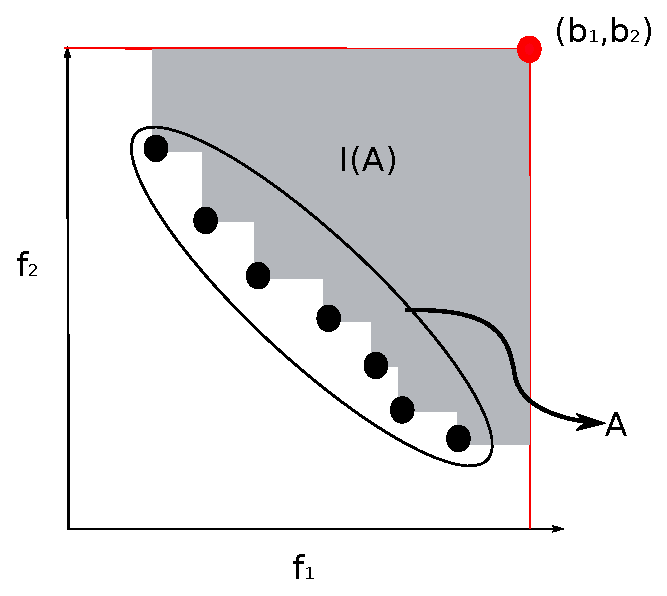
\includegraphics{hyperVol.eps}}
\end{minipage}
\begin{minipage}[b]{0.5\linewidth}
 \centering
 \resizebox*{9.0cm}{!}{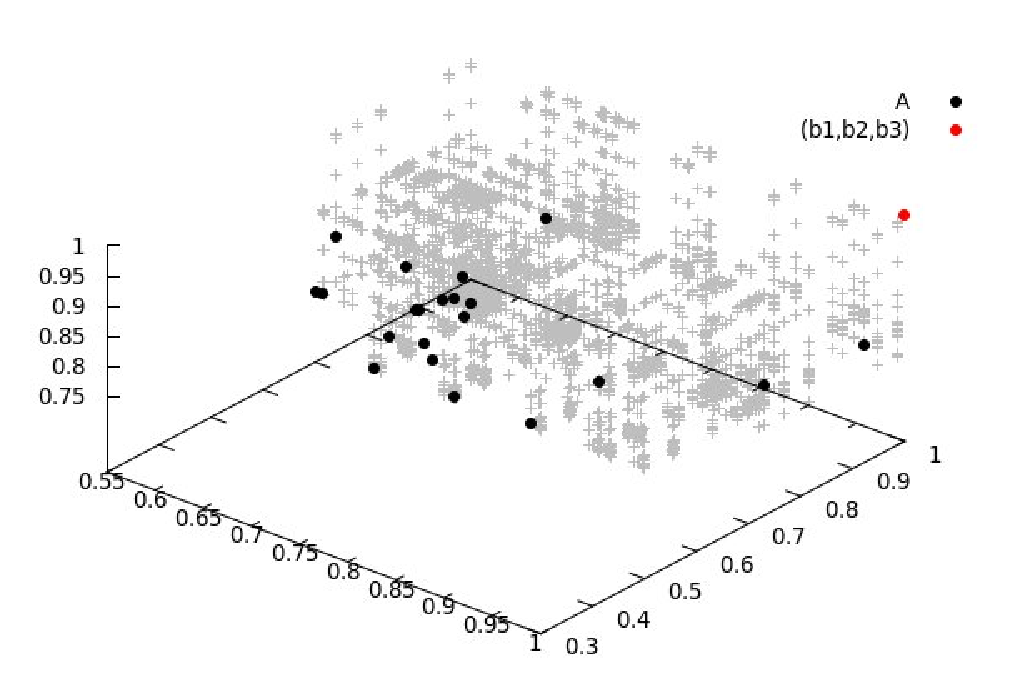
\includegraphics{pareto3d.eps}}
\end{minipage}
\caption{Two objective (left) and three objective (right) examples of hypervolume indicatror for set $A$. Reference point is $(b_1,...,b_M)$.}
\label{hyperV}
\end{figure}

Based on the same $\vec{b}$, two Pareto-fronts can be compared by computing their hypervolume indicators. Pareto front ($i$) is better from Pareto front ($j$) if the hypervolume indicator of ($i$) is grater that the hypervolume indicator of ($j$), namely 

\begin{eqnarray}
   i\prec j \leftrightarrow I(A_i,b) > I(A_j,b)
\end{eqnarray}    


\subsubsection{Constrained optimization problem}
EAs are not inherently built to handle constrained optimization problems. In engineering, though, all optimization problems are subject to a number of constraints, the most common ways to deal with constraints are a) the use of penalty functions \cite{Deb00,morales98} assigning evolutionary advantages to the individuals that satisfy the constraints \cite{powell93}, b) the conversion of constraints into objectives \cite{surry95,surry97} and c) the use of correction operators \cite{mich94}. Detailed literature survey on this subject can me found in \cite{mich96,coello02}.

In this thesis a penalty functions technique is in use. In the penalty functions technique EAs takes into account constraints by adding penalty terms (proportional to the magnitude of the constraint violation) on the cost function. For each constraint in addition to the hard limit ($d$, the constraint value as described by the optimization problem) a "relaxed limit" $d_k^*$ is also introduced. Once an individual violates the relaxed limit of one of the constraints ($c_k>d_k^*$) death penalty ($\Phi = \infty$) is given to it. If the individual violates one, or more, of the constraints ($c_k>d_k^*$) but none of the relaxed limits, a penalty is applied on it cost value $\Phi$. 

\begin{eqnarray}
	\Phi(\vec{x})=\Phi(\vec{x})+ \prod _{k=1}^K{\left\{ 				\begin{array}{ll}
    exp(a_k\frac{c_k(x)-d_k}{d_k^* -d_k}) & ~~,c_k(x)>d_k\\
    1 & ~~,c_k(x)\leq d_k\end{array} \right. }
    \label{penal2}
\end{eqnarray}  
where, $\vec{a}$ controls the penalization intensity for each individual constraint.

\begin{figure}[h!]
\begin{minipage}[b]{1.0\linewidth}
 \centering
 \resizebox*{10cm}{!}{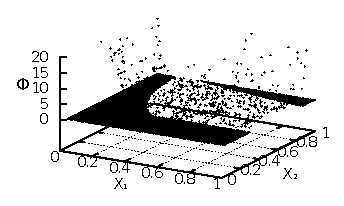
\includegraphics{fit_new.eps}}
\end{minipage}
\caption{$\Phi$ plot for 1000 randomly chosen individuals over the 2d design space of a two-objective constrained optimization problem (fig.\ref{case}) using the proposed penalization formulation (eq.\ref{penal2}).}
\label{fit2}
\end{figure}
 
\subsection{The $(\mu,\lambda)$EA}

The $(\mu,\lambda)$ EA used as the algorithmic basis of this thesis is described next.
Each generation $g$ of the $(\mu,\lambda)$EA is associated with three dynamically updated populations: the offspring $P_{\lambda}^g$ population containing $\lambda$ offsprings, the parent $P_{\mu}^g$ population containing $\mu$ parents and the elite $P_{e}^g$ population containing $e$ elites. $P_{e}^g$ contains the currently best individuals. Depending on variable coding (binary, binary grey or real), appropriate evolution operators should be applied. 

The $(\mu,\lambda)$ EA in use (cite Giotis 2003, na valo to elliniko didaktoriko?):
\begin{itemize}
\item[]{\bf Step 1:}  (Initialization) $g=0$, $P_{\mu}^g=0$ and $P_{\mu}^g=0$. All members of $P_{\lambda}^1$ are initialized using a, within the design bounds,  pseudo-random number generator. Injection of user defined individuals in the initial population is also possible. 
\item[]{\bf Step 2:}  (Evaluation) for every individual in $P_{\lambda}^g$, the vector $\vec{F}(\vec{x}) \in \Re^{M} $ is evaluated. In engineering problems evaluation is the most computationally demanding step.
\item[]{\bf Step 3:}  (Cost assignment) for each and every individual $\vec{x} \in P^g$ where, $P^g = P_{\lambda}^g \cup P_{\mu}^g \cup P_{e}^g$ a scalar cost $\Phi(\vec{x})$ value is assigned.
\item[]{\bf Step 4:}  (Elite selection) from population $P^*$ where $P^*=P_{\lambda}^g \cup P_{e}^{g-1}$ the $e^*$ not dominated individuals are selected to enter $P_e^g$. If $e^* > e$ a dilution operator is applied to remove $e^* - e$ neighbouring individuals.     
\item[]{\bf Step 5:}  (Elitism) a number of user-specified elite individuals replace the worst members of $P_{\lambda}^g$.  
\item[]{\bf Step 6:}  (Parent selection) Parent population is selected from $P_{\mu}^{g-1}$ , $P_{\lambda}^g$ taking into account the maximum generation limit (allowed age, in generations) $k$ for each parent. $P_{\mu}^{g}=S(P_{\mu}^{g-1},P_{\lambda}^g,k)$ 
\item[]{\bf Step 7:}  (Recombination and mutation) $P_{\lambda}^{g+1}$ is generated from 
$P_{\mu}^{g}$  by applying the recombination and mutation operators. Recombination $\mathcal{R}(P_{\mu}^{g})$ is the process of combining the genotype of $n$ parents to create a single offspring. The second step for the creation of $P_{\lambda}^{g+1}$ is the application of mutation operator. Mutation is the process that randomly changes one part of an individuals genotype $P_{\lambda}^{g+1} = \mathcal{M}(\mathcal{R}(P_{\mu}^{g}))$.
\item[]{\bf Step 8:}  (Finalise check) Unless a finalisation criteria is met, return to $step 2$.
\end{itemize}
Hereafter an evolutionary algorithm with $\mu$ parents and $\lambda$ offspring will be referred to as ($\mu,\lambda$)EA.   

\begin{table}[htdp]
\centering
\begin{tabular}{lr} 
\hline
\hline
number of objectives & M\\
number of design variables & N\\
number of constraints   & K\\
\hline
candidate solution   & x\\
objectives vector  & F\\
constraints vector  & C\\
cost value & $\Phi$ \\
\hline
\hline
\end{tabular}
\caption[GEA nomenclature]{($\mu,\lambda$)EA nomenclature}
\label{GEA nomenclature} 
\end{table}


\subsubsection{Evolution operators}
Evolution operators are the operators that evolve each generation to the next. This operators are namely; the parent selection operator, the recombination operator, the mutation operator and the elitism operator. This operators will be presented here.
   
\paragraph{Parent selection}
Parent selection aims at assigning to a selected group of individuals the ability to undergo recombination. The most common parent selection techniques are presented here; 
\begin{itemize}
\item[]{\bf a) Proportional selection.} Selection is based on assigning to each population member a probability to be a parent according to its cost value $\Phi$. This is implemented via a roulette wheel algorithm. Where each and every member of the population receives a slot of the roulette wheel, the size of the slot determines the probability to be a parent, and after $\mu$ spins the required $\mu$ parents are selected.  
\item[]{\bf b) Linear ranking.} In Linear ranking, the population is sorted according to $\Phi$ and placed in a sorted list. The probability to be a parent of each individual depends only on its position in the aforementioned list and not on the actual $\Phi$ value.
\item[]{\bf c) Probabilistic tournament selection.}
In probabilistic tournament selection \cite{goldberg1991}, a number of randomly chosen individuals are selected from the population and with a user defined, typically high, probability the best individual from this group is selected as parent. This process is repeated $\lambda$ times to create the required $\lambda$ parents. Parameters for tournament selection is the tournament size, how many individuals take place at each tournament and probability to select the best one. Typical values are $2$-$3$ individuals per tournament and $80\%$-$95\%$ probability to select the best.
\end{itemize}

\paragraph{Recombination}
Since the original formulation of EAs there has been numerous discussions about the merits of recombination as an evolution operator in EAs. In general the purpose of recombination in an EA is to increase the probability of offspring which are fitter than their parents \footnote{Simply put, recombination is the evolution operator that takes advantage of Schema theorem based building block hypothesis in order to increase the probability of offspring which are fitter than their parents.}. Recombination algorithms are separated in to two big groups, criterion being the coding of the design variables\footnote{Design variables in EAs can be represented either as strings of binary digits or a vector of real numbers.}, namely binary and real coding recombination algorithms.  

\subparagraph{Binary coding recombination} is based on exchanging pieces of the binary string that describes the design vector between the parents in order to create the offspring. Depending of the way this exchange takes place, the following types of binary coding recombination exists;
\begin{itemize}
\item[]{\bf a) One-point recombination.} 
In one point binary recombination for $\rho$ parents per offspring, the length of the binary string is divided into $\rho-1$ pieces corresponding to the number of possible pairings. The pairings take place between the lead parent and one of the remaining $\rho-1$ ones. For each of the aforementioned pairings a random integer $\mathcal{X}$ determines the crossover point\footnote{Analogous to biological crossover, crossing over point of chromosomes.}. The offspring is produced by receiving the left part of the string piece from one parent of the pairing and the right part from the other, this procedure repeated for all parings. A 2 parents example is presented below.
\begin{figure}[h!]
\begin{minipage}[b]{1.0\linewidth}
 \centering
 \resizebox*{10cm}{!}{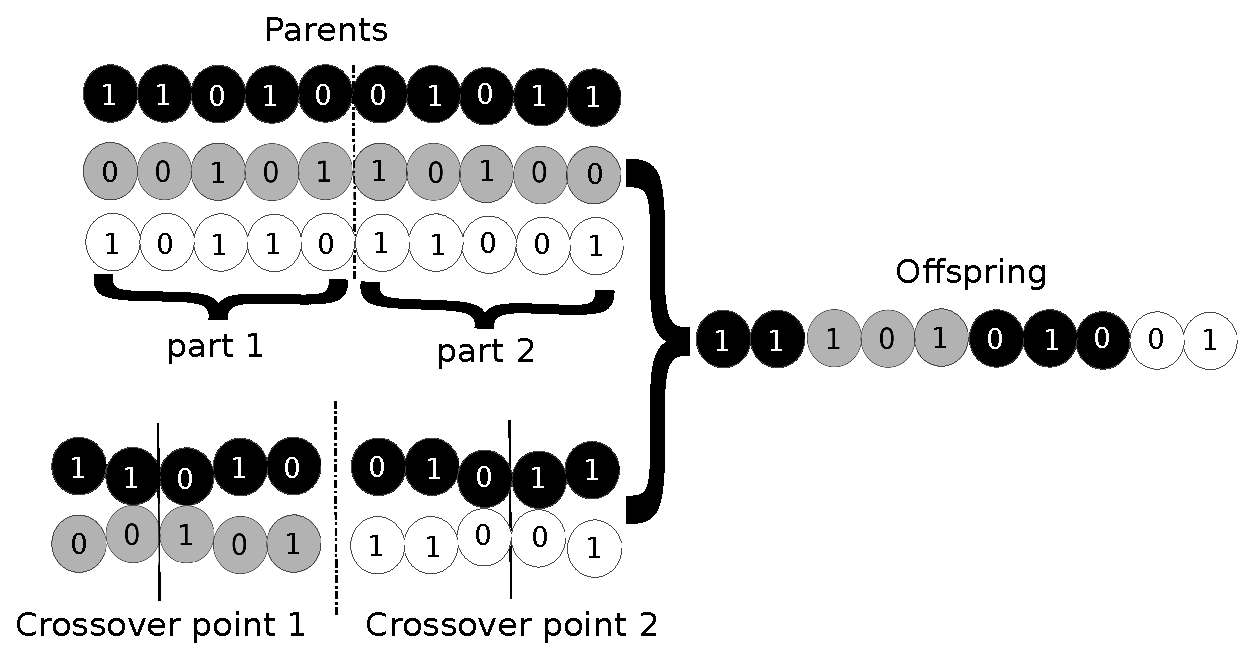
\includegraphics{onepointbinary.eps}}
\end{minipage}
\label{onepX}
\end{figure}
\pagebreak    
\item[]{\bf b) Two-point recombination}, shares the same algorithm as one point recombination only this time two crossover points are in use ($\mathcal{X}_1~\&~\mathcal{X}_2$).

\begin{figure}[h!]
\begin{minipage}[b]{1.0\linewidth}
 \centering
 \resizebox*{10cm}{!}{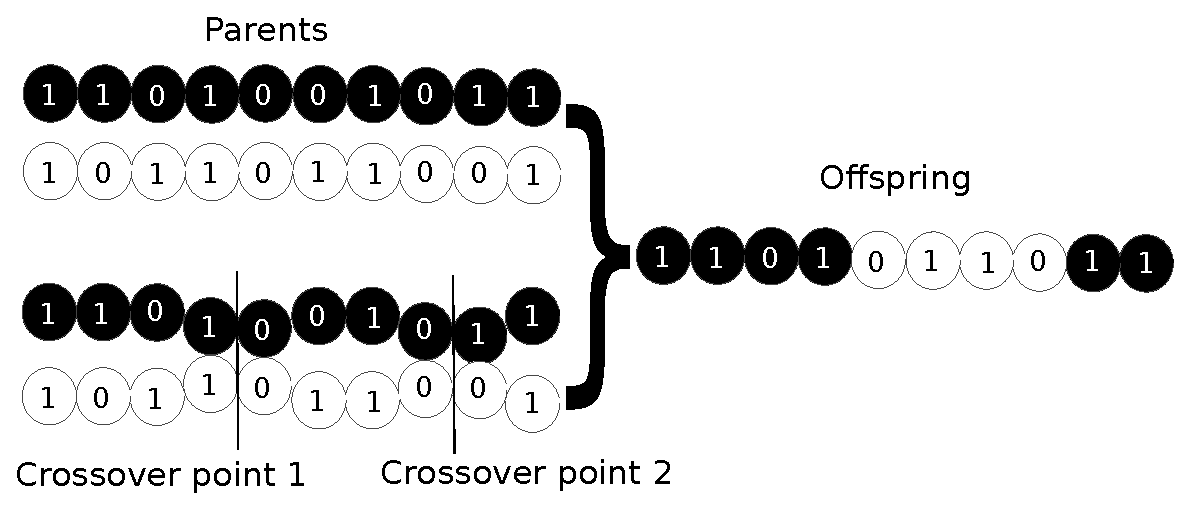
\includegraphics{twopointbinary.eps}}
\end{minipage}
\label{onepX}
\end{figure}

\item[]{\bf c) One or two point recombination per design variable}. Here the aforementioned one and two point recombination techniques are applied to the portions of the binary string that define each design variable separately.  
\end{itemize}
  

\subparagraph{Real coding recombination} using real coding representation of the design variables $\vec{x}$ allows the search over a continuous search space but also requires new recombination techniques that are applied not on the binary string, as for binary coating, but on the real-value design variables. The available real coding recombination types are listed below;  

\begin{itemize}
\item[]{\bf a) One point or two recombination.} The techniques of one and two point recombination as proposed for binary coding are transferred to real coding by exchanging  pieces of the design vector $\vec{x}$ instead of pieces of binary strings plus a mixing faction applied on the variables on the vicinity of the crossover point.

\begin{figure}[h!]
\begin{minipage}[b]{1.0\linewidth}
 \centering
 \resizebox*{10cm}{!}{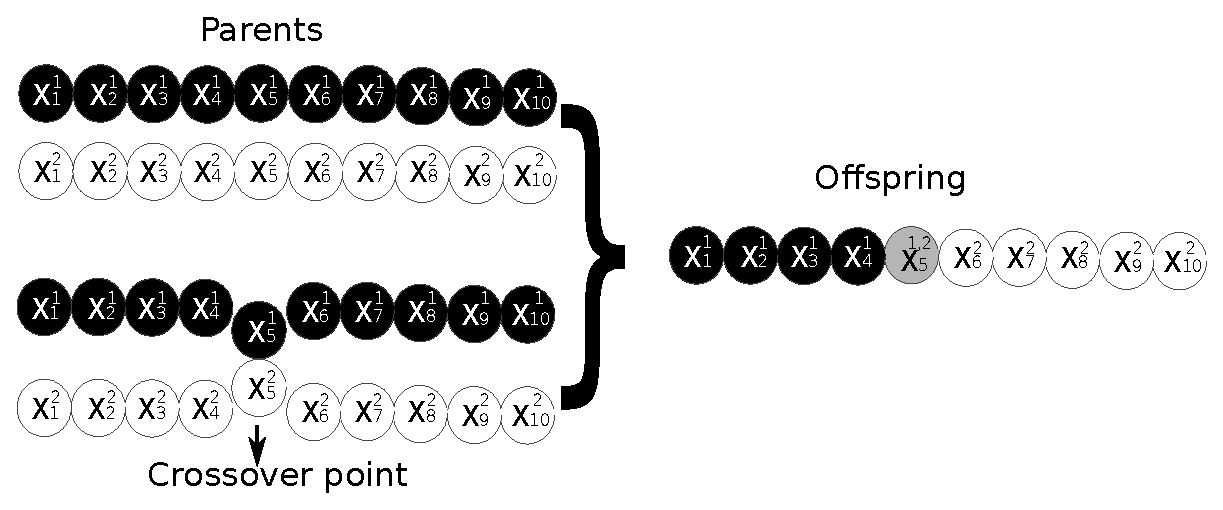
\includegraphics{pointreal.eps}}
\end{minipage}
\label{onepX}
\end{figure}
where, $x_5^{1,2}=x_5^{1}+r(x_5^{2}-x_5^{1}),~ r$ a random number uniformly distributed in $[0,1]$ ($r \in U(0,1)$).    
    
\item[]{\bf b) Discrete recombination.} In discrete recombination, each component of $\vec{x}$ for the offspring has $50\%$ probability to be copied either from the best parent $\vec{x}^1$ or a randomly chosen among the $\rho-1$ remaining ones $\vec{x}^{random}$. 

\begin{figure}[h!]
\begin{minipage}[b]{1.0\linewidth}
 \centering
 \resizebox*{10cm}{!}{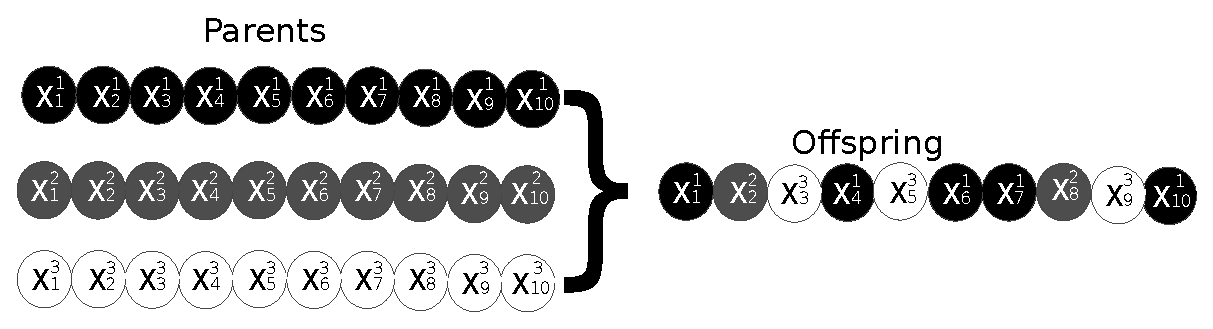
\includegraphics{discrete.eps}}
\end{minipage}
\label{onepX}
\end{figure}
where, $\vec{x^1}$ is the best parent.    
    
\item[]{\bf c) Generalized intermediate recombination}.  In generalized intermediate recombination, each component of $\vec{x}$ is a linear combination of $\vec{x}^1$ and a randomly chosen among the $\rho-1$ remaining ones $\vec{x}^{random}$.
\begin{eqnarray}
\nonumber
\vec{x}=\vec{x}^1+r(\vec{x}^{random}-\vec{x}^1),~ r\in U[0,1]
\end{eqnarray}  
 
\item[]{\bf d) Simulated binary crossover}. Simulated binary crossover (SBX) \cite{SBX1} was design with respect to one-point binary recombination properties of; a) average property \footnote{The average of the decoded parameter values is the same
before and after the crossover operation.} and b) spread factor property \footnote{The probability of occurrence of spread factor $\beta \approx 1$ is more likely than any other $\beta$ value. Spread factor $\beta$ has values close to one when the offspring are similar to the parents.}\cite{SBX1}. The offspring $\vec{x}$ is generated as follows;
\begin{eqnarray}
	\vec{x}={\left\{ 
	\begin{array}{ll}
    \vec{\overline{x}} - \frac{\beta}{2} (\vec{x}^{random}-\vec{x}^1)~~,\mbox{if $r < 0.5$}\\
	\vec{\overline{x}} + \frac{\beta}{2} (\vec{x}^{random}-\vec{x}^1)~~,\mbox{if $r \geq 0.5$}
    \end{array} \right. }
    \label{sbxx}
\end{eqnarray}  
where $r\in U[0,1]$, $\vec{\overline{x}}=mean(\vec{x}^{random},\vec{x}^1)$  and 
\begin{eqnarray}
	\beta={\left\{ 
	\begin{array}{ll}
    (2r)^{n}~~~~~~,\mbox{if $(r \leq 0.5)$}\\
	\left(\frac{1}{2r}\right)^{n+2}~~,\mbox{if $(r > 0.5)$}
    \end{array} \right. }
    \label{betasbx}
\end{eqnarray}

Since $r\in U[0,1]$, the probability distribution of $\beta$ can be plotted for various $n$ based on eq.\ref{betasbx} (fig.\ref{sbx}-left). Based on the $\beta$ probability distribution and eq.\ref{sbxx} the probability distribution of offspring as a function of $n$ and the parents can be plotted (fig.\ref{sbx}-right for a 1d problem and fig.\ref{sbx2} for a 2d problem). In general higher $n$ values cause higher probability of $\beta \approx 1$ which leads to hight probability of offspring being similar to their parents (spread factor property). Together with the symmetrical offspring probability distribution with respect to $\vec{\overline{x}}$ (average property) "SBX" can simulate the one point binary crossover ergo.    

\begin{figure}[h!]
\begin{minipage}[b]{0.5\linewidth}
 \centering
 \resizebox*{7cm}{!}{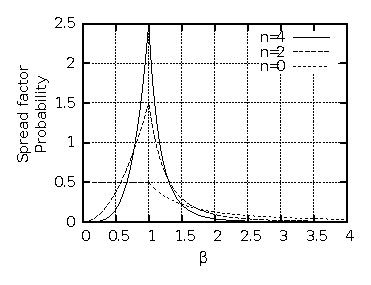
\includegraphics{SBX.eps}}
\end{minipage}
\begin{minipage}[b]{0.5\linewidth}
 \centering
 \resizebox*{7cm}{!}{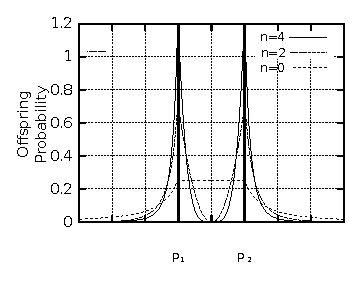
\includegraphics{SBXparents.eps}}
\end{minipage}
\caption{Left: the probability distribution of $\beta$ is plotted for various $n$. Increasing $n$ leads to higher probability of $\beta \approx 1$. Right: the offspring probability distribution of a 1D problem is plotted as a function of the parents $P_1$ and $P_2$ and the value of $n$ }
\label{sbx}
\end{figure}

\begin{figure}[h!]
\begin{minipage}[b]{0.5\linewidth}
 \centering
 \resizebox*{7cm}{!}{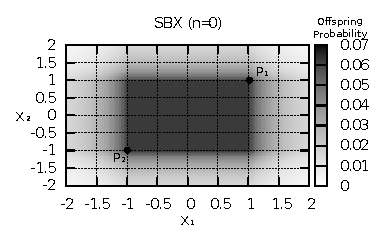
\includegraphics{SBX3dparents0.eps}}
\end{minipage}
\begin{minipage}[b]{0.5\linewidth}
 \centering
 \resizebox*{7cm}{!}{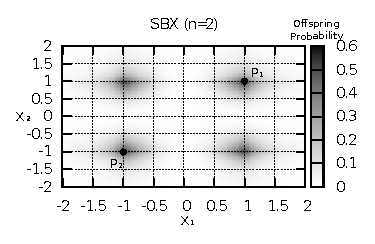
\includegraphics{SBX3dparents2.eps}}
\end{minipage}
\caption{The offspring probability distribution of a 2D optimization problem, two parent ($P_1(1,1)$ \& $P_2(-1,-1)$) recombination is plotted for $n=0$ left and $n=2$ right.}
\label{sbx2}
\end{figure}
\end{itemize}
  
\paragraph{Mutation}
The purpose of mutation in an EA scheme is to introduce and preserve diversity in the population. Thus mutation prevents the population of chromosomes from becoming too similar to each other, thus slowing or even stopping/stagnating the evolution. Mutation is applied to each offspring resulted from the recombination, subject to a small mutation probability $P_m$. Mutation, as recombination, is also categorized in two groups according with the design variable coding.     

\subparagraph{Binary coding mutation.} In binary coding mutation, $P_m$ is applied on each and every bit of the binary string that represents the individual. For each bit of the binary string there is a probability $P_m$ to switch state from 0 to 1, or vice versa.      

\begin{figure}[h!]
\begin{minipage}[b]{1\linewidth}
 \centering
 \resizebox*{10cm}{!}{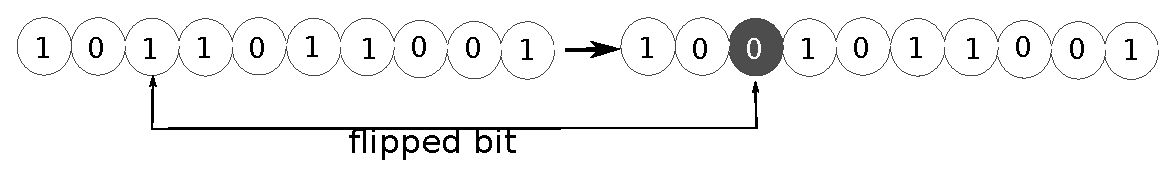
\includegraphics{mut.eps}}
\end{minipage}
\label{binarymut}
\end{figure}

\subparagraph{Real coding mutation.} In real coding mutation $P_m$ is applied on each member of $\vec{x}$. 

\begin{eqnarray}
	\vec{x}_m={\left\{ 
	\begin{array}{ll}
    \vec{x}~~~~~~~~~~,\mbox{if $(P_m > r)$}\\
	M(\vec{x},D)~,\mbox{if $(P_m \leq r)$}
    \end{array} \right. }
    \label{}
\end{eqnarray}
where $r\in U[0,1]$ and

\begin{eqnarray}
	M(\vec{x},D)={\left\{ 
	\begin{array}{ll}
    \vec{x}+D(g,\vec{U}-\vec{x})~\mbox{if $(r_1 > 0.5)$}\\
	\vec{x}-D(g,\vec{x}-\vec{L})~\mbox{if $(r_1 \leq r)$}
    \end{array} \right. }
    \label{}
\end{eqnarray}
where, $r_1\in U[0,1]$, $\vec{U}$ and $\vec{L}$ the vectors of upper and lower bounds of the design space accordingly and  

\begin{eqnarray}
   D(g,y) = y r_2 (1-g/g_{max})^{0.2}
\end{eqnarray}

where $g_{max}$ the number of maximum generations and $r_2\in U[0,1]$.

%\begin{eqnarray}
%	\vec{\sigma}=\frac{min(\mid \vec{x}-\vec{UB}\mid,\mid \vec{x}- \vec{LB}\mid)}{3} * (1-\frac{g}{g_{max}})^p
%	\label{sigmamut} 
%\end{eqnarray}
%where $\vec{UB}$ and $\vec{LB}$ the vectors of upper and lower bounds for the design variables respectively. $g$ the current generation and $g_{max}$ the maximum allowed generations.$p \simeq 0.2$.

%The first part of the eq.\ref{sigmamut} ensures that the mutated individual will respect the design variable bounds and the second part reduces exponentially eith $p$ the magnitude of $\vec{\sigma}$ as the generations advance.

%\begin{figure}[h!]
%\begin{minipage}[b]{0.5\linewidth}
% \centering
% \resizebox*{7cm}{!}{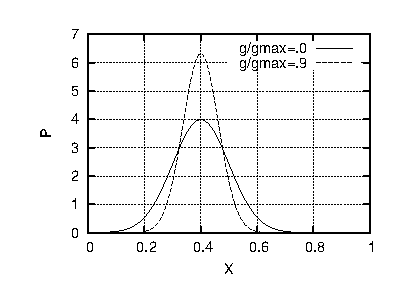
\includegraphics{Mut_1d.eps}}
%\end{minipage}
%\begin{minipage}[b]{0.5\linewidth}
% \centering
% \resizebox*{8cm}{!}{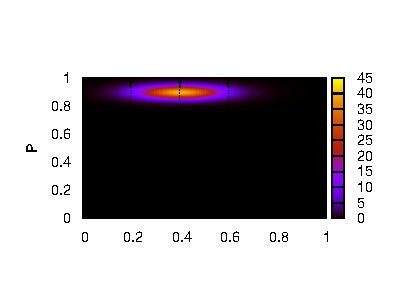
\includegraphics{Mut_2d.eps}}
%\end{minipage}
%\label{realmut}
%\caption{Examples of mutant probability distributions for one design variable left $x=0.4$ and two design variable right $\vec{x}=(0.4,0.9)$. For both cases $\vec{LB}=0$ and $\vec{UB}=1$.}
%\end{figure}

\paragraph{Elitism}
The purpose of elitism in EAs is to guarantee a mononously improoving course of evolution \cite{Back1996}. In the EA used as algorithmic basis for the thesis elitism operator was generalize with the use of a separate population $P_e^g$ that gets updated every generation as described in ($\mu,\lambda$)EA-step:4. Furthermore a number of user-specified elite individuals replace the worst members of the offspring population $P^g_{\lambda}$ before the parent selection operator takes place.
  

\subsection{Metamodel assisted Evolutionary Algorithm}

Due to the involvement of costly evaluation tools (such as CFD tools to numerically predict flows in or around complex 3D geometries), solving engineering optimization problems using EAs may become very computationally demanding. The extensive, smart use of low-cost surrogate evaluation models (often referred to as "metamodels") during the optimization decreases substantially the number of calls to the computationally expensive, problem-specific evaluation code (CFD) making EAs a viable tool that can routinely be used to solve large-scale industrial optimization problems, with affordable wall clock time. Literature surveys on the use of metamodels within EAs can be found in papers \cite{LTT_2_020,Jin2002,LTT_2_027} or books \cite{KEANEbook}.


Polynomial regression, artificial neural networks, Gaussian processes etc. have all been used as metamodels.  Schemes based on different interactions between the metamodel and the problem-specific evaluation tool have been published. Hereafter, all of them will be referred to as MAEAs. This thesis uses the MAEA presented in \cite{LTT_2_018} for SOO and \cite{LTT_2_029} for MOO. 

For all but the first few generations, the metamodels are used to pre-evaluate the current population. Based on the outcome of approximate pre-evaluations, a few most promising individuals are identified and these solely undergo evaluation on the problem-specific evaluation tool to compute their "exact" objective function value(s), before proceeding to the next generation. The $(\mu,\lambda)$ MAEA used herein is sketched in fig.~\ref{MAEA}.


\begin{figure}[h!]
\centering
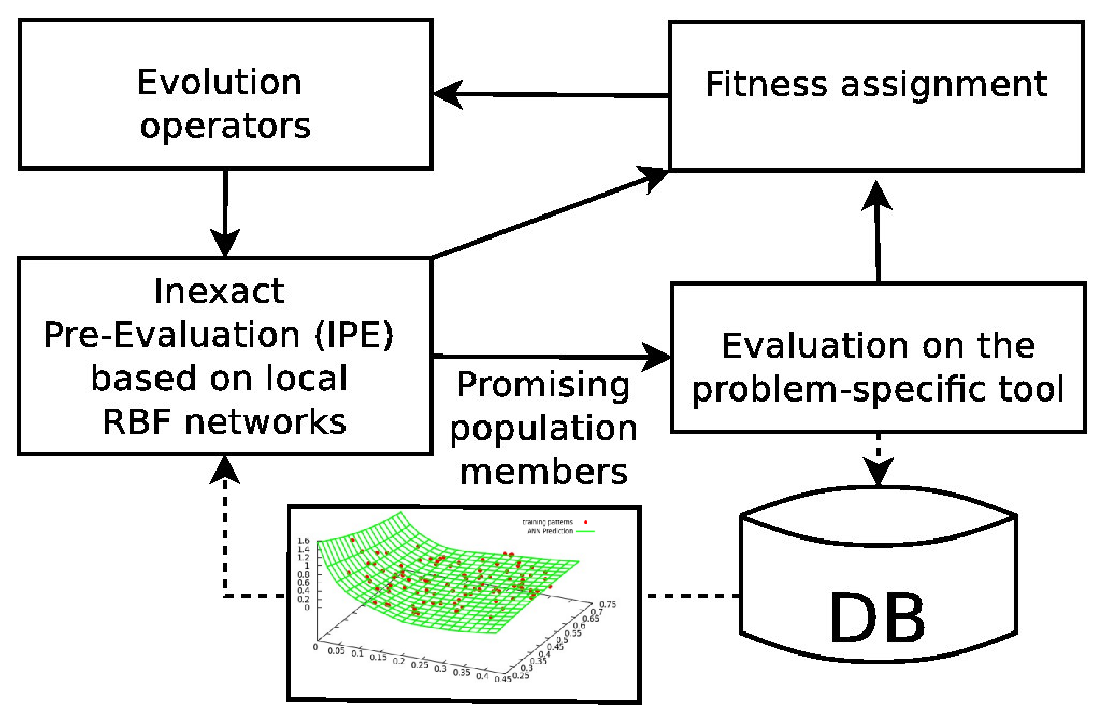
\includegraphics[width=90mm]{MAEA.eps} 
\caption{Schematic representation of the MAEA (namely the variant using on-line trained metamodels) this paper relies on. The loop corresponds to a single EA generation. The so-called inexact pre-evaluation (IPE) phase, within the EA--based search, is used, as described in \cite{LTT_2_020,LTT_2_029}. }
\label{MAEA}
\end{figure}


\paragraph{Radial Basis Function networks enhanced by importance factors}
Herein Radial Basis Function networks (RBFn) are used as metamodels. RBFn are multilayer artificial neural networks (ANN) with three layers, (input,hidden and output) as shown in fig.\ref{rbf1} \cite{Haykin}. Signals propagate through the network in the forward direction, from the input to the output layer, by performing a nonlinear mapping (eq.\ref{RBFa}) followed by a linear one. The latter is related to the weight coefficients $w_l$ that must be computed during the training on a number of available patterns. An RBF network to be used within a MAEA should have $N$ input units, i.e. as many as the  design variables. The hidden layer includes $L$ nodes, associated with the so–called RBF centers $c^l$. At each hidden neuron a nonlinear mapping of the input signals to a single value is carried out using the radial-basis activation function $G:\Re^N \rightarrow \Re$, acting on the distance of input $x$ (eq.\ref{RBFa}) from the corresponding center $c^l \in \Re^N$.  In the current thesis the Gaussian activation is in use. 

\begin{eqnarray}
	G(u,r)=exp(\frac{-u^2}{r^2})
	\label{RBFa}
\end{eqnarray}  
where $u=\Vert x-c^l \Vert_2$ the distance from the corresponding $l^{th}$ RBF center.

\begin{figure}[h!]
\centering
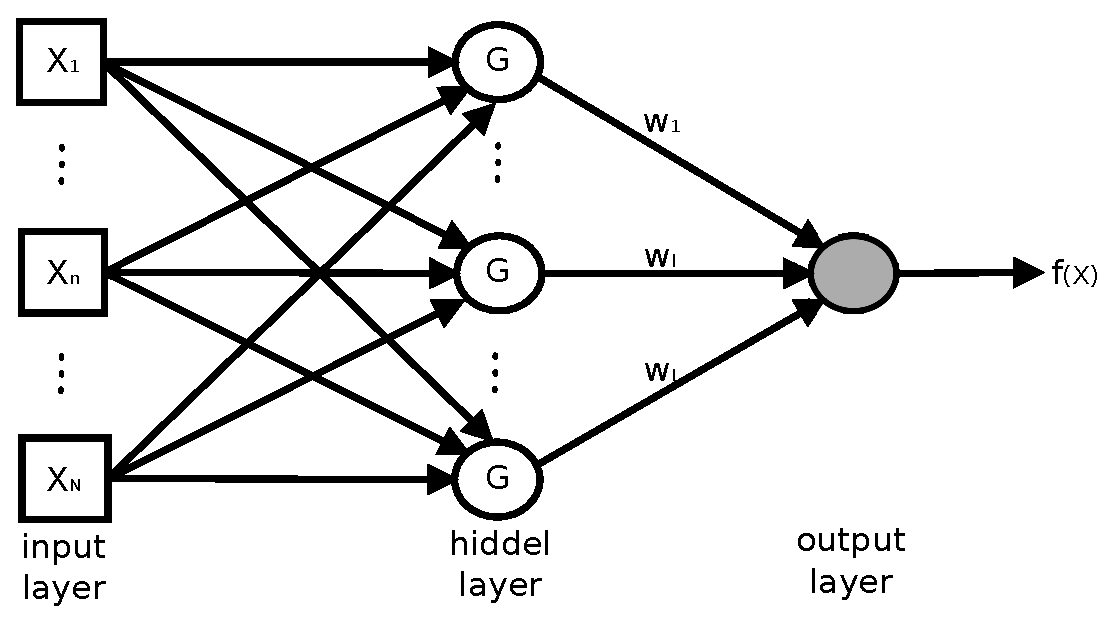
\includegraphics[width=90mm]{RBF.eps} 
\caption{Radial basis function network.}
\label{rbf1}
\end{figure}
The values that the radii or widths r take on may considerably affect the prediction abilities of the network; these are computed using heuristics,\cite{Haykin}. The output layer includes as many nodes as the responses of the network. The single response we are dealing with is expressed by the sum of the weighted output signals from the hidden neurons, as follows             
\begin{eqnarray}
	f(x)=\sum _1^N w_i*G(u(x_i),r)
\end{eqnarray}  


\subsection{Hierarchical Evolutionary Algorithm}
Typically in engineering design a number of tools with different fidelity and cost (computational and/or economical) are available and used in different steps of the design procedure (fig.\ref{HMAEA} right). Relatively fast low fatality tools are used in the initial stages of the design in order to efficiently scan the design space and high fatality slow (and/or expensive with respect to licensed software or laboratory time) tools are used for the latter steps of design for fine-tuning. In case of turbo-machinery design, for example, a potential code can be used as a low fidelity tool followed by dense or coarse grid Euler codes, Navier-Stokes codes for a single flow passage or the full machine and finally actual laboratory test and adaptation cycles.    


\begin{figure}[h!]
\begin{minipage}[b]{1.0\linewidth}
 \centering
 \resizebox*{13cm}{!}{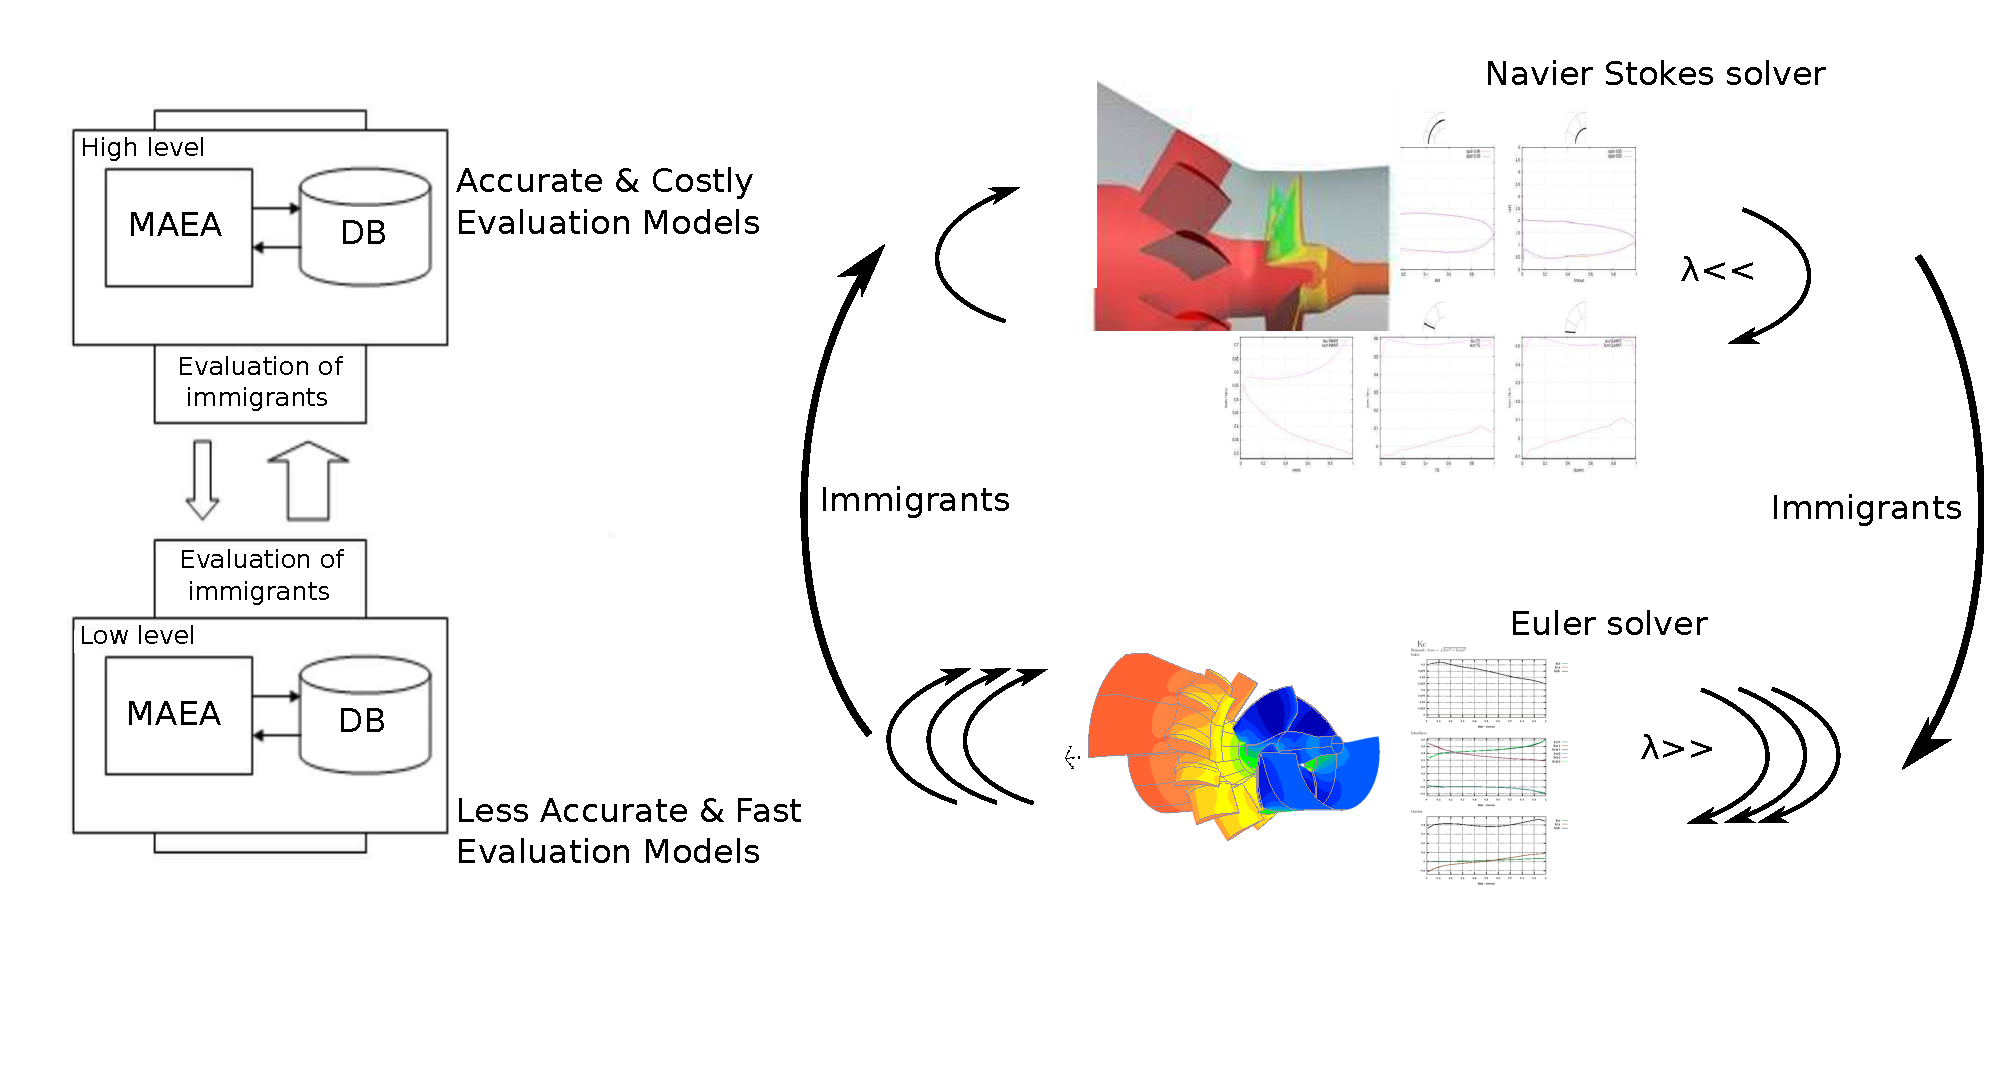
\includegraphics{handmade.eps}}
\end{minipage}
\caption{Left, schematic representation of a two level HMAEA (Hierarchical metamodel assisted evolutionary algorithm). High level is associated with the expensive and accurate tool and lower level with the cheap but not so accurate tool. Communication between the two level is possible in both directions including re-evaluation with the receiving levels evaluation tool. Right, example of two level design procedure as used in industry. A relatively big number of designs is evaluated with the Euler solver once a good design is located it is evaluated with the Navier-Stokes solver. Possible faults are identified, targets for the lower level are updated, that would result in the  elimination of the aforementioned faults, bye experienced designers.}
\label{HMAEA}
\end{figure} 
 
In order to exploit the availability of this tools Hierarchical evolutionary algorithms (HEA) where devised (cite Kampolis + papers). HEA are enhanced EA variants which utilise a number of evolution Levels, each level assigned a different evaluation tool (fig.\ref{HMAEA} left). This multilevel search mechanism splits the computational burden among the levels. On the lower levels, a low cost exploration of the search space is carried out through global search methods, less demanding or less accurate evaluation tools or by even using reduced design variable sets, etc. On the other hand the higher levels undertake the fine-tuning part of the design procedure through denser parameterization, more accurate evaluation tools and/or stochastic or deterministic search methods. These levels mainly serve to refine immigrants from the lower levels. Intercommunication and two-way migrations of individuals between adjacent levels are necessary. The number of levels, the frequency of migration and the number of immigrants are user-defined parameters.

% ---------------------------------------------------------------------------
% ----------------------- end of thesis sub-document ------------------------
% ---------------------------------------------------------------------------